%%%%%%%%%%%%%%%%%%%%%%%%%%%%%%%%%%%%%%%%%%%%
% Chapitre 9
%%%%%%%%%%%%%%%%%%%%%%%%%%%%%%%%%%%%%%%%%%%%

\chapter{Influence du cadre statistique sur des méthodes basées tenseurs}
\label{Chapter9}



% \minitoc

%----------------------------------------------------------------------------------------

\section{Évaluation de la variété géométrique utilisée}
La \figref{fig:res_manifold} présente les différents résultats obtenus pour la comparaison entre les métriques des variétés Euclidienne, Log-Euclidienne et Riemmanienne.
D'une part, ils mettent en évidence que les performances de ces méthodes varient suivant le type de lésion simulée.
La méthode \textit{GLM-DT} surpasse les deux autres pour détecter une diminution de la diffusion longitudinale.
D'autre part, les méthodes \textit{GLM-LOG-DT} et \textit{MGLM-DT} montrent des résultats légèrement supérieurs 
pour détecter des lésions produits par une augmentation de la diffusion radiale.
Il faut aussi noter que ces trois méthodes présentent des performances similaires pour la détection des deux autres types de lésions 
(une modification de l'orientation de la diffusion et une augmentation de la diffusion moyenne).
Enfin, nous remarquons que les méthodes utilisant des métriques Log-Euclidienne et Riemmanienne mènent à des résultats particulièrement similaires.

\begin{figure*}[t]
    \centering
    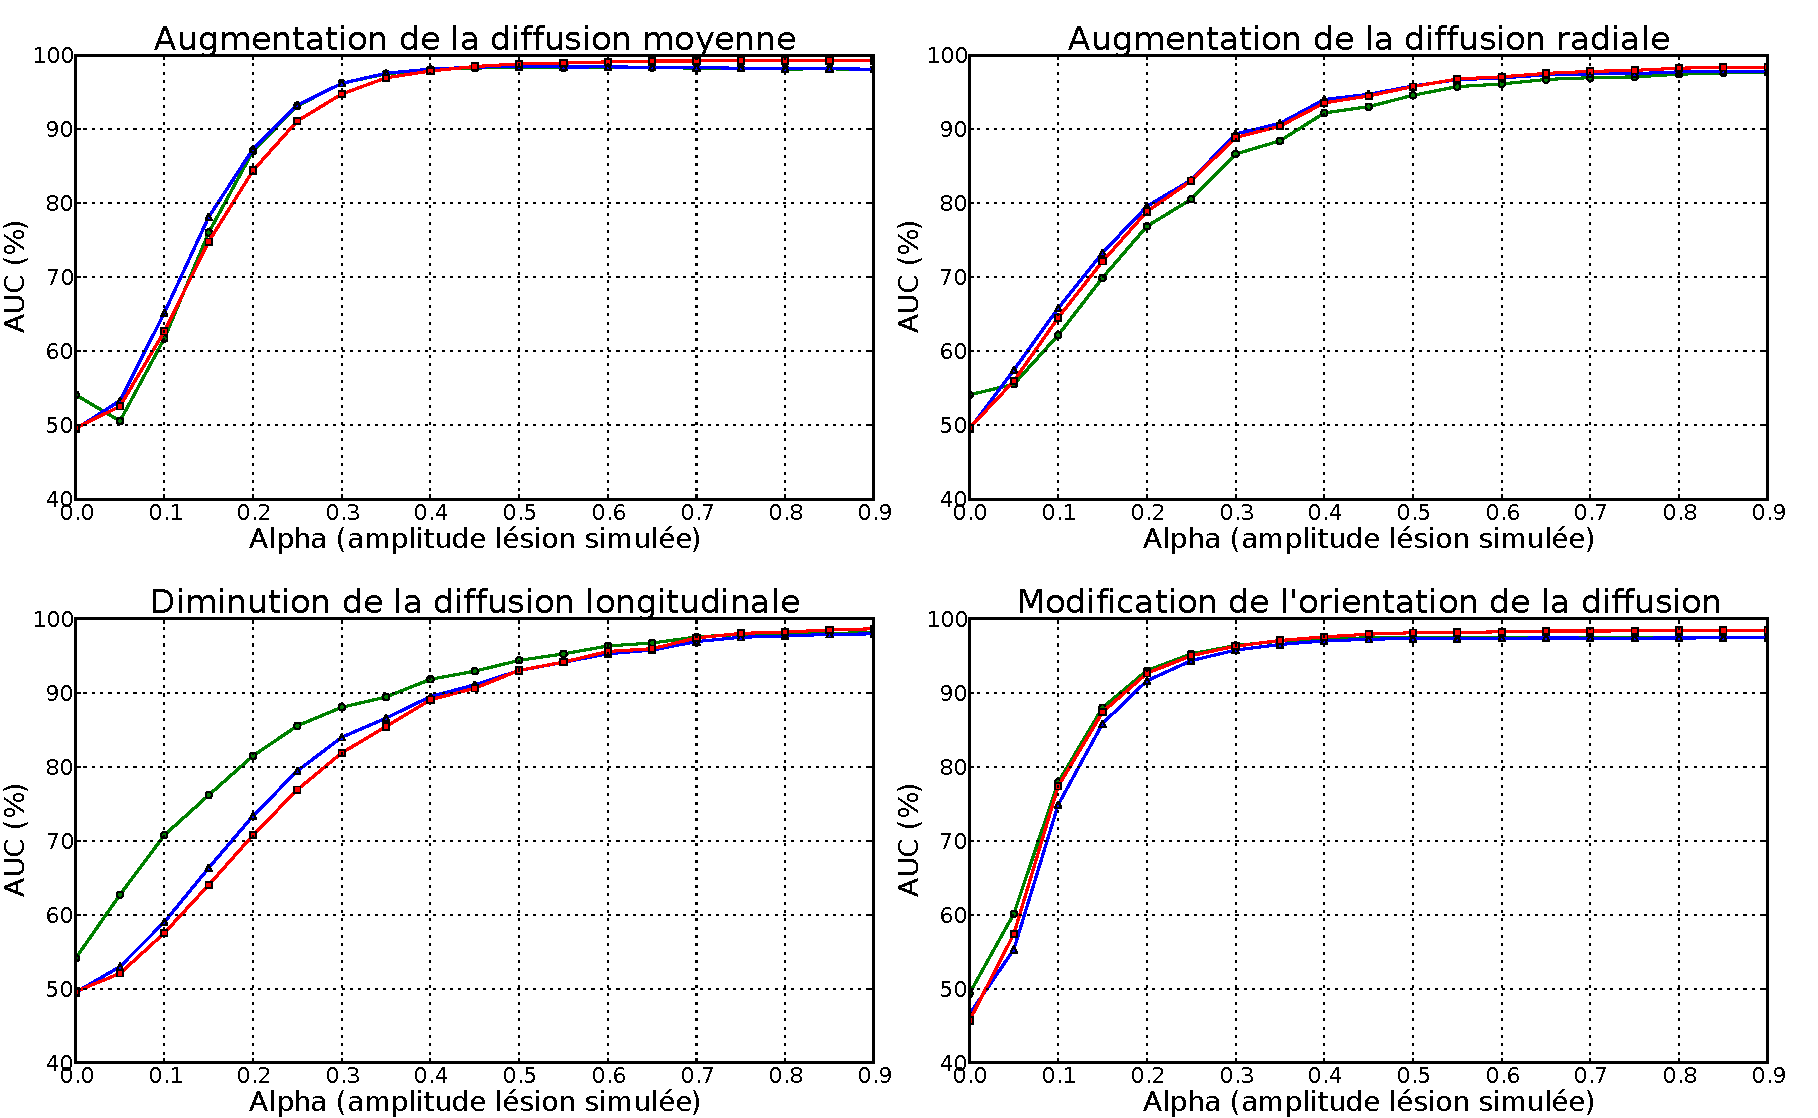
\includegraphics[width=1\textwidth]{Images/AUC_frameworks_gaussian8_fr.pdf}
    \caption{\label{fig:res_manifold} Influence de la variété géométrique ({\color{green} $\bullet$ = GLM-DT},  {\color{blue} $\blacktriangle$ = GLM-LOG-DT}, {\color{red} $\blacksquare$ = MGLM-DT}).}
\end{figure*}


\section{Discussion}

In the literature, a few works have already evaluated the impact of the Euclidean, Log-Euclidean and affine invariant-Riemannian metrics
 for various images processing problems \cite{Arsigny2006, Pasternak2010} but there is still no consensus on the most appropriate manifold for handling diffusion tensors, 
especially in the context of group comparison.
Some papers prone the use of  Log-Euclidean or Riemannian metrics for conducting DT-MRI group comparison \cite{Zhu2009, Schwartzman2010, Yuan2012, Kim2014}.
Some other papers claim that these metrics are not superior \cite{Whitcher2007} or even inferior \cite{Pasternak2010} to the Euclidean one. In their comparison between Euclidean
and Log-Euclidean metrics, Whitcher \textit{et al}  \cite{Whitcher2007} conclude that there is no reason to prefer the log-Euclidean distance and that
applying matrix logarithms to diffusion tensors tends to reduce the group difference observed in Euclidean space.
Moreover, both theoretic analysis and experimental results reported in \cite{Pasternak2010} support that the Euclidean metric is more appropriate than an affine-invariant metric for the analysis of diffusion coefficients and tensors.

Our experimental results on simulated lesions highlight that all metrics can efficiently detect every kind of lesions,
with performance varying for each framework according to the kind of simulated change.
The results on the real database confirm the good ability of the three metrics to detect the regions
involved in the NMO, without exhibiting any significant difference between the detection maps.
Regarding the computational burden (\tabref{tab:cpu_time}), 
the typical computation time for conducting the statistical analysis of the NMO database on a standard workstation 
is about 2 min for the Euclidean and Log-Euclidean approaches as compared to about 80 hours for the Riemannian framework. 
This time gap may probably be reduced by optimizing the implementation of the Riemannian framework\footnote{\url{https://www.nitrc.org/projects/riem\_mglm}},
for instance by rewriting the MATLAB code in C++ language.
But in any case, the Riemannian framework would still be much more computationally intensive than the Euclidean and Log-Euclidean approaches.


\begin{table}[htbp]
\centering
\begin{tabular}{|D{4cm}|D{4cm}|}
      \hline
      \textbf{Méthodes} & \textbf{Temps d'exécution ($s$)} \tabularnewline
      \hline
      GLM-FA & 135 \tabularnewline
      GLM-MD & 135 \tabularnewline
      GLM-DT & 135 \tabularnewline
      GLM-LOG-DT & 148 \tabularnewline
      MGLM-DT & 253392 \tabularnewline
      \hline
  \end{tabular}
  \caption{\label{tab:cpu_time} Temps d'exécution en $s$ pour les analyses statistiques de la base NMO.}
\end{table}

In conclusion, this study suggests that, despite the mathematical elegance offered by the Riemannian framework, its superiority on both simulated and real clinical data could not be demonstrated compared to the Euclidean and Log-Euclidean frameworks. 
For a similar performance, these two latter methods present the advantage to be easily implementable and computationally effective. This conclusion is of course limited to the scope of the present application. 
